% The seventh roots of unity; the six chords from 1 have product of lengths 7 (generated by a script).
\begin{tikzpicture}[scale=1.0]
\draw[black!25,->] (-2.6,0)--(2.9,0); \draw[black!25,->] (0,-2.5)--(0,2.6);
\draw[black!40] (0,0) circle (2.0);
\draw[MidnightBlue!50,thin] (2.000,0.000)--(1.247,1.564)--(-0.445,1.950)--(-1.802,0.868)--(-1.802,-0.868)--(-0.445,-1.950)--(1.247,-1.564)--cycle;
\draw[Orange!90!black,thick] (2.000,0.000)--(1.247,1.564);
\draw[Orange!90!black,thick] (2.000,0.000)--(-0.445,1.950);
\draw[Orange!90!black,thick] (2.000,0.000)--(-1.802,0.868);
\draw[Orange!90!black,thick] (2.000,0.000)--(-1.802,-0.868);
\draw[Orange!90!black,thick] (2.000,0.000)--(-0.445,-1.950);
\draw[Orange!90!black,thick] (2.000,0.000)--(1.247,-1.564);
\fill[MidnightBlue] (2.000,0.000) circle (0.06);
\node[font=\small] at (2.400,0.000) {$1$};
\fill[MidnightBlue] (1.247,1.564) circle (0.06);
\node[font=\small] at (1.496,1.876) {$\zeta$};
\fill[MidnightBlue] (-0.445,1.950) circle (0.06);
\node[font=\small] at (-0.534,2.340) {$\zeta^{2}$};
\fill[MidnightBlue] (-1.802,0.868) circle (0.06);
\node[font=\small] at (-2.162,1.041) {$\zeta^{3}$};
\fill[MidnightBlue] (-1.802,-0.868) circle (0.06);
\node[font=\small] at (-2.162,-1.041) {$\zeta^{4}$};
\fill[MidnightBlue] (-0.445,-1.950) circle (0.06);
\node[font=\small] at (-0.534,-2.340) {$\zeta^{5}$};
\fill[MidnightBlue] (1.247,-1.564) circle (0.06);
\node[font=\small] at (1.496,-1.876) {$\zeta^{6}$};
\node[font=\small,align=left,anchor=west] at (2.9,1.4) {$|1-\zeta|\,|1-\zeta^2|\cdots|1-\zeta^6|=\Phi_7(1)=7$};
\node[font=\small,align=left,anchor=west] at (2.9,0.6) {$|1-\zeta|=2\sin\frac\pi7\approx0.868$};
\node[font=\small,align=left,anchor=west] at (2.9,-0.2) {$\dfrac{1-\zeta^a}{1-\zeta}$ is a unit for $7\nmid a$};
\node[font=\small,align=left,anchor=west] at (2.9,-1.1) {so $7\mathcal O=(1-\zeta)^6$};
\end{tikzpicture}
